\documentclass[aspectratio=169]{beamer}
% ----- Pacotes -----
\usepackage{tikz}
\usepackage{xcolor}
\usepackage{amsmath}
\usepackage{listings}
\usepackage{biblatex}
\usepackage{graphicx}
\usepackage{fontspec}
\usepackage[brazil]{babel}
% ----- Fontes -----
\setmainfont{Fira Sans}
\setmonofont{Fira Code}
% ----- Configuração do Pacote Listings -----
\usetheme{Madrid}
\definecolor{keywordcolor}{rgb}{0.6, 0.1, 0.6}
\definecolor{commentcolor}{rgb}{0.3, 0.6, 0.3}
\definecolor{stringcolor}{rgb}{0.8, 0.1, 0.1}
\definecolor{bgcolor}{rgb}{0.95, 0.95, 0.95}
\definecolor{identifiercolor}{rgb}{0.1, 0.1, 0.9}
\lstset{
    keywords={sudo, apt, dnf, pacman, brew, install, winget},
    keywordstyle=\color{keywordcolor}\bfseries,
    ndkeywords={gnupg, gpg, gen-key, import, export, list-keys, encrypt, sign, verify, Gpg4win},
    ndkeywordstyle=\color{identifiercolor}\bfseries,
    comment=[l]{\#},
    commentstyle=\color{commentcolor}\itshape,
    stringstyle=\color{stringcolor},
    morestring=[b]",
    morestring=[b]',
    identifierstyle=\color{black},
    backgroundcolor=\color{bgcolor},
    basicstyle=\ttfamily\footnotesize,
    showstringspaces=false,
    breaklines=true,
    captionpos=b,
    frame=single,
    rulecolor=\color{black},
}
% ----- Configurações do Documento -----
\date{\today}
\addbibresource{refs.bib}
\logo{
\includegraphics[width=1cm]{figuras/brasao.png}}
\title[GNU Privacy Guard]{Seminário - Redes II: GnuPG}
\author[Hernane\and Gustavo\and João\and Matheus\and Pedro]{
    Hernane Velozo Rosa \and
    Gustavo Valadares Castro \and
    João Víctor Martins Medeiros \and\\
    Matheus Dias Soares \and
    Pedro Igor Martins dos Reis
}
\institute[PUC]{Pontifícia Universidade Católica de Minas Gerais}
% ----- Documento -----
\begin{document}
\begin{frame}
	\maketitle
\end{frame}
\section{Sobre o projeto}
\subsection{Introdução}
\begin{frame}
	\frametitle{Introdução}
	\begin{itemize}
		\item \textbf{GnuPG} (\textit{GNU Privacy Guard}) é uma ferramenta gratuita e de código aberto para criptografia e assinatura de dados \cite{gnupgPrivacyGuard};
		\item Se propõe a garantir a privacidade e a autenticidade das comunicações digitais \cite{archlinuxGnuPGArchWiki};
		\item Desenvolvido como uma alternativa ao PGP (\textit{Pretty Good Privacy});
		\item Parte do projeto \textbf{GNU}, seguindo os princípios do software livre.
	\end{itemize}
\end{frame}
\subsection{Uso do Software}
\begin{frame}[fragile]
	\frametitle{Instalação e Configuração}
	\begin{lstlisting}[caption=Comandos para instalação]
brew install gnupg                      # MacOS
winget install -h gnupg.Gpg4win         # Windows 10/11
sudo {apt,dnf,pacman,...} install gnupg # Distribuições Linux
        \end{lstlisting}
\end{frame}
\subsection{Casos de Uso}
\begin{frame}[fragile]
	\frametitle{Exemplos de uso}
	\begin{lstlisting}[caption=Parâmetros úteis]
gpg --gen-key                           # Gerar chave;
gpg --import chave.pub                  # Importar chave;
gpg --export -a "nome" > chave.pub      # Exportar chave;
gpg --list-keys                         # Listar chaves;
gpg -e -r "recipient" arquivo           # Criptografar arquivo;
gpg --sign arquivos                     # Gerar assinatura;
gpg --verify arquivo.assinado           # Verificar assinatura.
        \end{lstlisting}
\end{frame}
\begin{frame}
	\frametitle{Exemplos de uso}
	\begin{figure}[ht!]
		\centering
		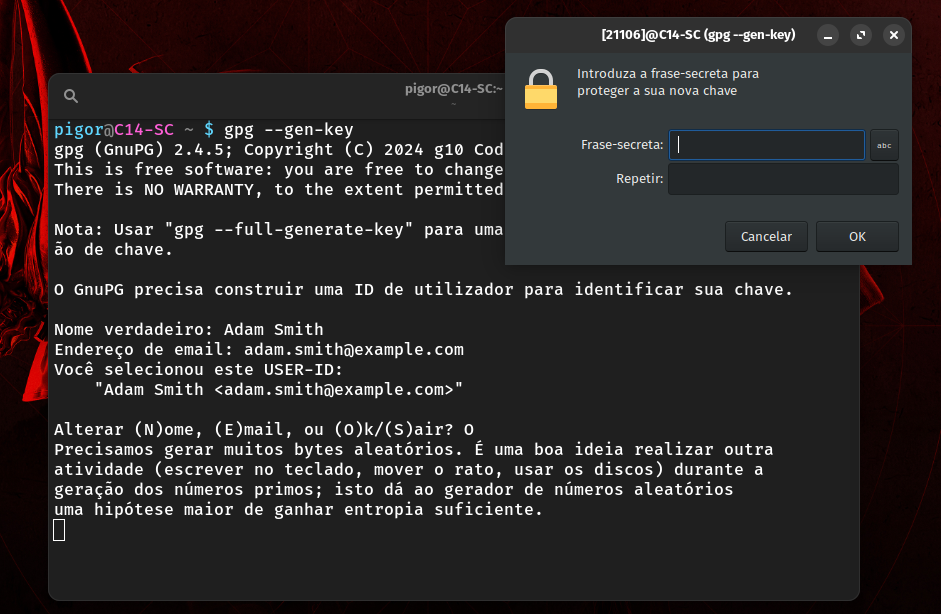
\includegraphics[width=0.6\textwidth]{figuras/genkey.png}
		\caption{Comando '--gen-key' em execução.}
	\end{figure}
\end{frame}
\begin{frame}[fragile]
	\begin{lstlisting}[caption=Saída de exemplo]
gpg: pasta '/home/ad-smith/.gnupg/openpgp-revocs.d' criada
gpg: certificado de revogação armazenado como '...F015906A9083E.rev'
chaves pública e privada criadas e assinadas.

pub   ed25519 2024-05-31 [SC] [expira: 2027-05-31]
      CCEBE16CFA1F1958058FB4BC1C8F015906A9083E
uid   Adam Smith <adam.smith@example.com>
sub   cv25519 2024-05-31 [E] [expira: 2027-05-31]
\end{lstlisting}
\end{frame}
\begin{frame}
	\frametitle{Funcionalidade}
	\begin{itemize}
		\item Criptografa arquivos e mensagens para proteger contra acesso não autorizado;
		\item Confirma a origem e integridade dos dados recebidos;
		\item Garante a autenticidade e integridade dos dados;
		\item E-mails, documentos, arquivos sensíveis;
		\item Uso em sistemas de controle de versão \cite{lucas2006pgp} para assinar \textit{commits} (ex.: Git).
	\end{itemize}
\end{frame}
\section{Desvantagens}
\begin{frame}
\begin{figure}
\centering
\begin{tikzpicture}
\draw[thick,->] (0,0) -- (6,0) node[anchor=north] {\textbf{Comportamento}};
\draw[thick,->] (0,0) -- (0,6) node[anchor=south] {\textbf{Qualidade}};

\draw[dashed] (0,0) -- (6,6);
\draw[dashed] (0,6) -- (6,0);
\draw[dashed] (0,3) -- (6,3);
\draw[dashed] (3,0) -- (3,3);
\draw[dashed] (0,6) -- (6,6);

\node[anchor=north] at (3,6) {Sup. Ataque};
\node[anchor=south] at (3,3) {Ponto Crítico};

\draw[thick,smooth,variable=\x,domain=0:6] plot ({\x},{-1/3*(\x-3)^2+3});
\end{tikzpicture}
\end{figure}
\end{frame}
\section{Questão}
\begin{frame}
	\frametitle{Enunciado}
	O GnuPG (GNU Privacy Guard) é uma ferramenta amplamente utilizada para criptografia e assinatura digital de dados. No entanto, há situações onde o uso do GnuPG pode não ser a escolha mais prática. Em qual dos cenários abaixo o uso do GnuPG provavelmente não seria prático?
	\begin{itemize}
		\item a) Envio de documentos sensíveis por e-mail entre duas empresas que já possuem chaves públicas trocadas e configuradas.
		\item b) Criptografia de arquivos armazenados em um servidor compartilhado, acessível por vários funcionários que possuem chaves públicas compatíveis.
		\item c) Troca de mensagens instantâneas em tempo real entre duas pessoas usando um aplicativo de bate-papo.
		\item d) Assinatura digital de documentos para garantir a autenticidade e integridade ao enviar para clientes que utilizam GnuPG.
	\end{itemize}
\end{frame}
\begin{frame}
	\frametitle{Gabarito}
	O GnuPG (GNU Privacy Guard) é uma ferramenta amplamente utilizada para criptografia e assinatura digital de dados. No entanto, há situações onde o uso do GnuPG pode não ser a escolha mais prática. Em qual dos cenários abaixo o uso do GnuPG provavelmente não seria prático?
	\begin{itemize}
		\item a) Envio de documentos sensíveis por e-mail entre duas empresas que já possuem chaves públicas trocadas e configuradas.
		\item b) Criptografia de arquivos armazenados em um servidor compartilhado, acessível por vários funcionários que possuem chaves públicas compatíveis.
		\item \textcolor{green}{\textbf{c) Troca de mensagens instantâneas em tempo real entre duas pessoas usando um aplicativo de bate-papo.}}
		\item d) Assinatura digital de documentos para garantir a autenticidade e integridade ao enviar para clientes que utilizam GnuPG.
	\end{itemize}
\end{frame}
\subsection{Fontes Utilizadas}
\begin{frame}
	\frametitle{Referências}
	\printbibliography
\end{frame}
\end{document}
